\documentclass[]{tufte-book}

% ams
\usepackage{amssymb,amsmath}

\usepackage{ifxetex,ifluatex}
\usepackage{fixltx2e} % provides \textsubscript
\ifnum 0\ifxetex 1\fi\ifluatex 1\fi=0 % if pdftex
  \usepackage[T1]{fontenc}
  \usepackage[utf8]{inputenc}
\else % if luatex or xelatex
  \makeatletter
  \@ifpackageloaded{fontspec}{}{\usepackage{fontspec}}
  \makeatother
  \defaultfontfeatures{Ligatures=TeX,Scale=MatchLowercase}
  \makeatletter
  \@ifpackageloaded{soul}{
     \renewcommand\allcapsspacing[1]{{\addfontfeature{LetterSpace=15}#1}}
     \renewcommand\smallcapsspacing[1]{{\addfontfeature{LetterSpace=10}#1}}
   }{}
  \makeatother

\fi

% graphix
\usepackage{graphicx}
\setkeys{Gin}{width=\linewidth,totalheight=\textheight,keepaspectratio}

% booktabs
\usepackage{booktabs}

% url
\usepackage{url}

% hyperref
\usepackage{hyperref}

% units.
\usepackage{units}


\setcounter{secnumdepth}{2}

% citations
\usepackage{natbib}
\bibliographystyle{apalike}

% pandoc syntax highlighting

% longtable
\usepackage{longtable,booktabs}

% multiplecol
\usepackage{multicol}

% strikeout
\usepackage[normalem]{ulem}

% morefloats
\usepackage{morefloats}


% tightlist macro required by pandoc >= 1.14
\providecommand{\tightlist}{%
  \setlength{\itemsep}{0pt}\setlength{\parskip}{0pt}}

% title / author / date
\title{Improving the Reproducibility of Experimental Data Recording and Pre-Processing}
\author{Brooke Anderson, Michael Lyons, Mercedes Gonzalez-Juarrero, Marcela Henao-Tamayo, and Gregory Robertson}
\date{}

\usepackage{booktabs}
\usepackage{amsthm}
\usepackage{fontspec}
    \setmainfont{Gill Sans}
\makeatletter
\def\thm@space@setup{%
  \thm@preskip=8pt plus 2pt minus 4pt
  \thm@postskip=\thm@preskip
}
\makeatother

\begin{document}

\maketitle



{
\setcounter{tocdepth}{1}
\tableofcontents
}

\hypertarget{overview}{%
\chapter{Overview}\label{overview}}

\newthought{The recent NIH-Wide Strategic Plan} \citep{nih2016strategic}
describes an integrative view of biology and human health that includes
translational medicine, team science, and the importance of capitalizing on an
exponentially growing and increasingly complex data ecosystem \citep{nih2018data}.
Underlying this view is the need to use, share, and re-use biomedical data
generated from widely varying experimental systems and researchers. Basic
sources of biomedical data range from relatively small sets of measurements,
such as animal body weights and bacterial cell counts that may be recorded by
hand, to thousands or millions of instrument-generated data points from various
imaging, -omic, and flow cytometry experiments. In either case, there is a
generally common workflow that proceeds from measurement to data recording,
pre-processing, analysis, and interpretation. However, in practice the distinct
actions of data recording, data pre-processing, and data analysis are often
merged or combined as a single entity by the researcher using commercial or open
source spreadsheets, or as part of an often proprietary experimental measurement
system / software combination (Figure \ref{fig:workflow}), resulting in key
failure points for reproducibility at the stages of data recording and
pre-processing.

\begin{figure*}

{\centering 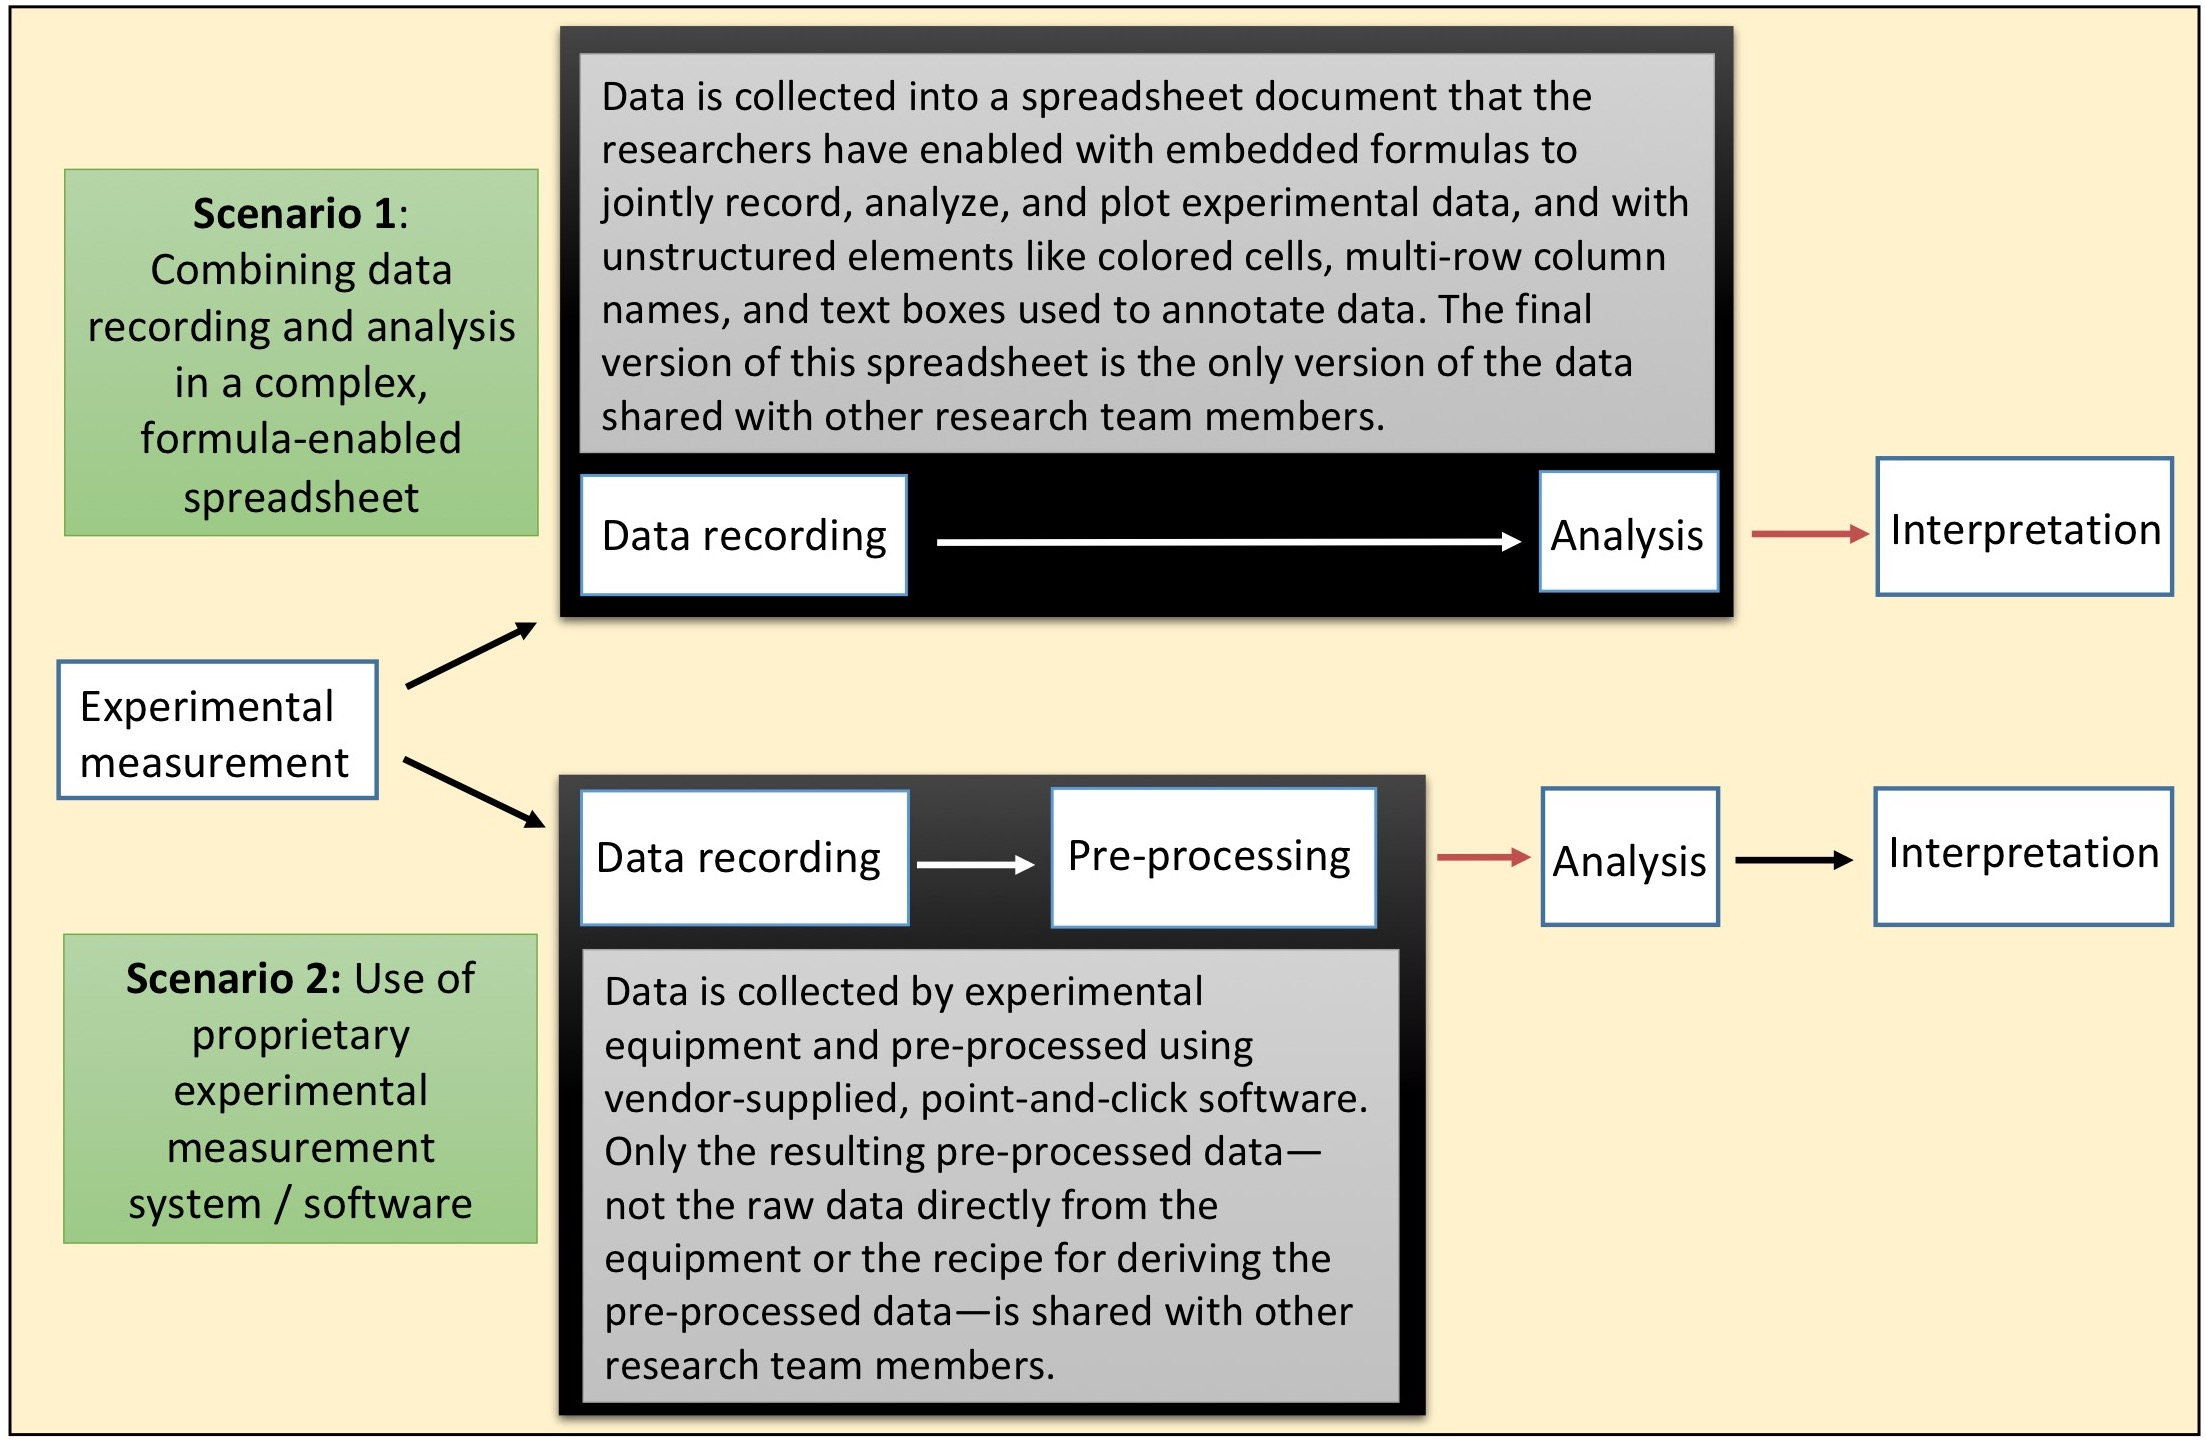
\includegraphics[width=30.64in]{figures/existing_blackboxes} 

}

\caption[Two scenarios where 'black boxes' of non-transparent, non-reproducible data handling exist in research data workflows at the stages of data recording and pre-processing]{Two scenarios where 'black boxes' of non-transparent, non-reproducible data handling exist in research data workflows at the stages of data recording and pre-processing. These create potential points of failure for reproducible research. Red arrows indicate where data is passed to other research team members, including statisticians / data analysts, often within complex or unstructured spreadsheet files.}\label{fig:workflow}
\end{figure*}

It is widely known and discussed among data scientists, mathematical modelers,
and statisticians \citep{broman2018data, krishnan2016towards} that there is
frequently a need to discard, transform, and reformat various elements of the
data shared with them by laboratory-based researchers, and that data is often
shared in an unstructured format, increasing the risks of introducing errors
through reformatting before applying more advanced computational methods.
Instead, a critical need for reproducibility is for the transparent and clear
sharing across research teams of: (1) raw data, directly from hand-recording or
directly output from experimental equipment; (2) data that has been
pre-processed as necessary (e.g., gating for flow cytometry data, feature
identification for metabolomics data), saved in a consistent, structured format,
and (3) a clear and repeatable description of how the pre-processed data was
generated from the raw data \citep{broman2018data, ellis2018share}.

To enhance data reproducibility, it is critical to create a clear separation
among data recording, data pre-processing, and data analysis---breaking up
commonly existing ``black boxes" in data handling across the research process.
Such a rigorous demarcation requires some change in the conventional
understanding and use of spreadsheets and a recognition by biomedical
researchers that recent advances in computer programming languages, especially
the R programming language, provide user-friendly and accessible tools and
concepts that can be used to extend a transparent and reproducible data workflow
to the steps of data recording and pre-processing. Among our team, we have found
that there are many common existing practices---including use of spreadsheets
with embedded formulas that concurrently record and analyze experimental data,
problematic management of project files, and reliance on proprietary,
vendor-supplied point-and-click software for data pre-processing---that can
interfere with the transparency, reproducibility, and efficiency of
laboratory-based biomedical research projects, problems that have also been
identified by others as key barriers to research reproducibility
\cite{broman2018data, bryan2018excuse, ellis2018share, marwick2018packaging}. In
these training modules, we have choosen topics that tackle barriers to
reproducibility that have straightforward, easy-to-teach solutions, but which
are still very common in biomedical laboratory-based research programs.

Click on the \textbf{Next} button (or navigate using the
links at the top of the page) to continue.

\hypertarget{experimental-data-recording}{%
\chapter{Experimental Data Recording}\label{experimental-data-recording}}

\hypertarget{separating-data-recording-and-analysis}{%
\section{Separating data recording and analysis}\label{separating-data-recording-and-analysis}}

\hypertarget{subsection-1}{%
\subsection{Subsection 1}\label{subsection-1}}

\hypertarget{subsection-2}{%
\subsection{Subsection 2}\label{subsection-2}}

\hypertarget{principles-and-power-of-structured-data-formats}{%
\section{Principles and power of structured data formats}\label{principles-and-power-of-structured-data-formats}}

\hypertarget{subsection-1-1}{%
\subsection{Subsection 1}\label{subsection-1-1}}

\hypertarget{subsection-2-1}{%
\subsection{Subsection 2}\label{subsection-2-1}}

\hypertarget{the-tidy-data-format}{%
\section{The `tidy' data format}\label{the-tidy-data-format}}

\hypertarget{subsection-1-2}{%
\subsection{Subsection 1}\label{subsection-1-2}}

\hypertarget{subsection-2-2}{%
\subsection{Subsection 2}\label{subsection-2-2}}

\hypertarget{designing-templates-for-tidy-data-collection}{%
\section{Designing templates for `tidy' data collection}\label{designing-templates-for-tidy-data-collection}}

\hypertarget{subsection-1-3}{%
\subsection{Subsection 1}\label{subsection-1-3}}

\hypertarget{subsection-2-3}{%
\subsection{Subsection 2}\label{subsection-2-3}}

\hypertarget{experimental-data-pre-processing}{%
\chapter{Experimental Data Pre-Processing}\label{experimental-data-pre-processing}}

\bibliography{book.bib,packages.bib}



\end{document}
